\chapter{Implementation}\label{appendix_implementation}
\begin{figure}[h!]
	\centering
	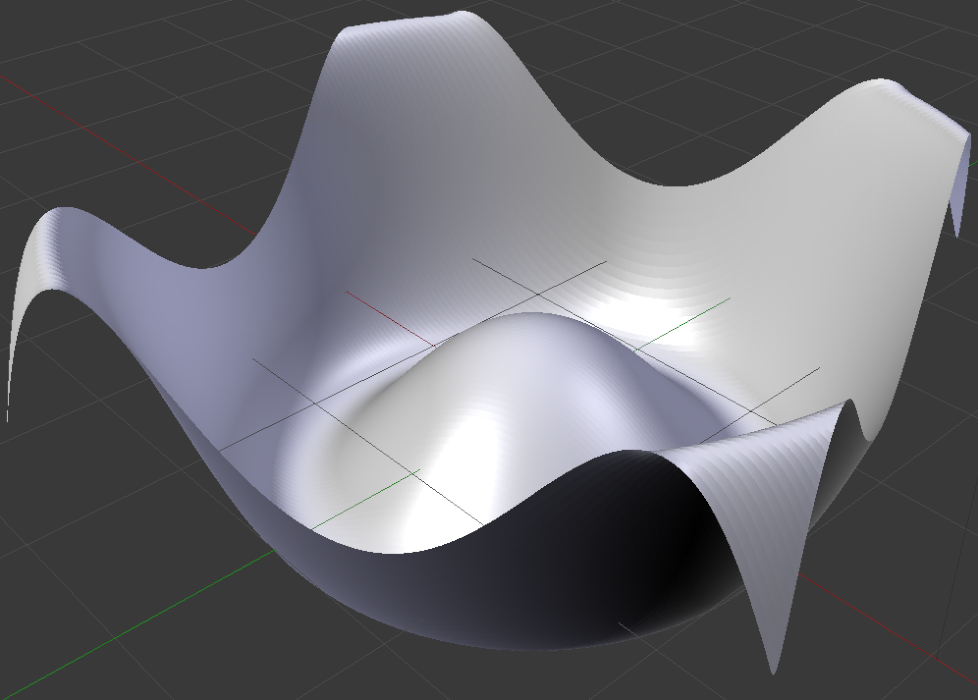
\includegraphics[height=5cm]{images/sil_viewport.png}
	\caption{Initial object, defined in Blender, and displayed in the Blender viewport.}\label{sil_viewport}
\end{figure}

\FloatBarrier
\section{Silhouette}\label{impl_silhouette}
\begin{figure}[h!]
	\centering
	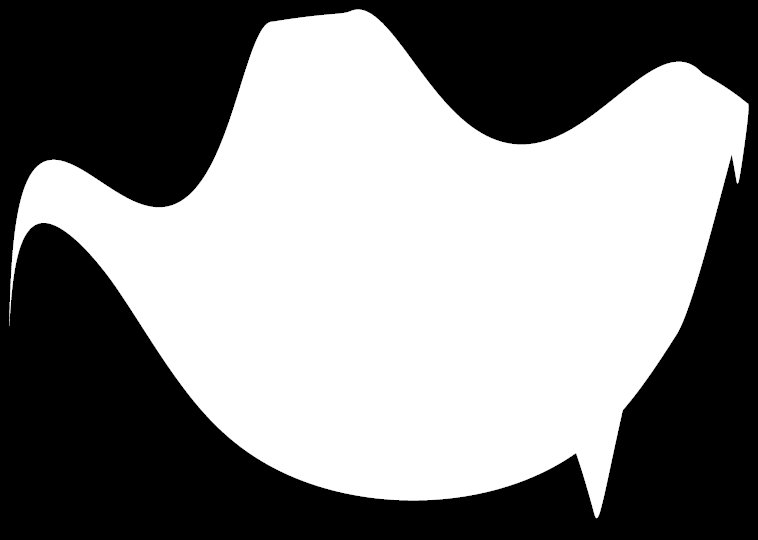
\includegraphics[height=5cm]{images/sil_obj.png}
	\caption{Object index pass produced by Cycles.}\label{sil_obj}
\end{figure}

\begin{figure}[h!]
	\centering
	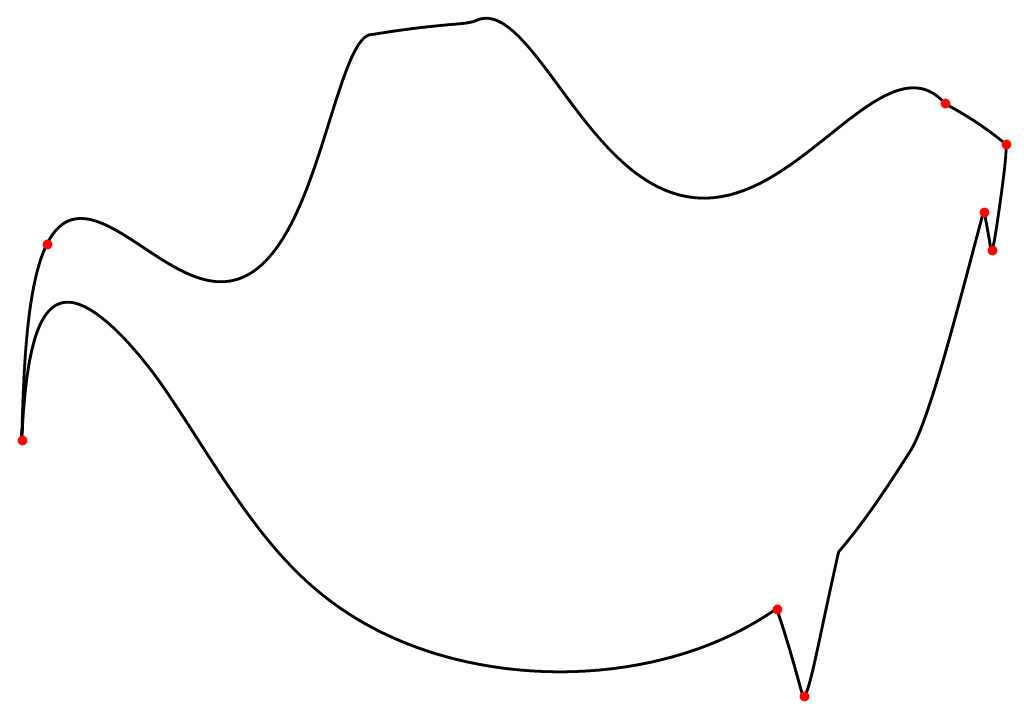
\includegraphics[height=5cm]{images/sil_path_corners.png}
	\caption{Silhouette \texttt{Path} and sharp edges identified.}\label{sil_path_corners}
\end{figure}

\begin{figure}[h!]
	\centering
	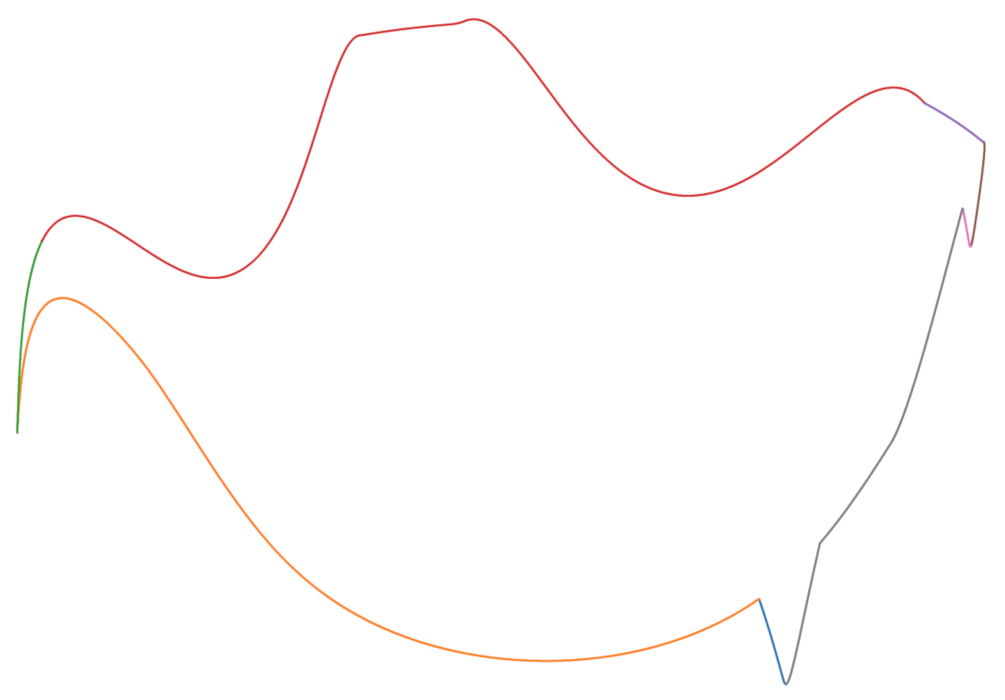
\includegraphics[height=5cm]{images/sil_split_paths.png}
	\caption{Silhouette \texttt{Path} split into multiple \texttt{Path}s based on sharp edges. A \texttt{Curve1D} object is created for each \texttt{Path}, which produces a composite Bezier curve definition for each segment.}\label{sil_split_paths}
\end{figure}

\begin{figure}[h!]
	\centering
	\includesvg[height=5cm]{images/sil.svg}
	\caption{\texttt{Path}s converted to \texttt{CurvedStroke}s, and rendered as a SVG. Thickness at each line location is proportional to distance from the camera (perspective foreshortening).}\label{sil_obj}
\end{figure}

\FloatBarrier
\section{Internal Edges}\label{impl_internal}
\begin{figure}[h!]
	\centering
	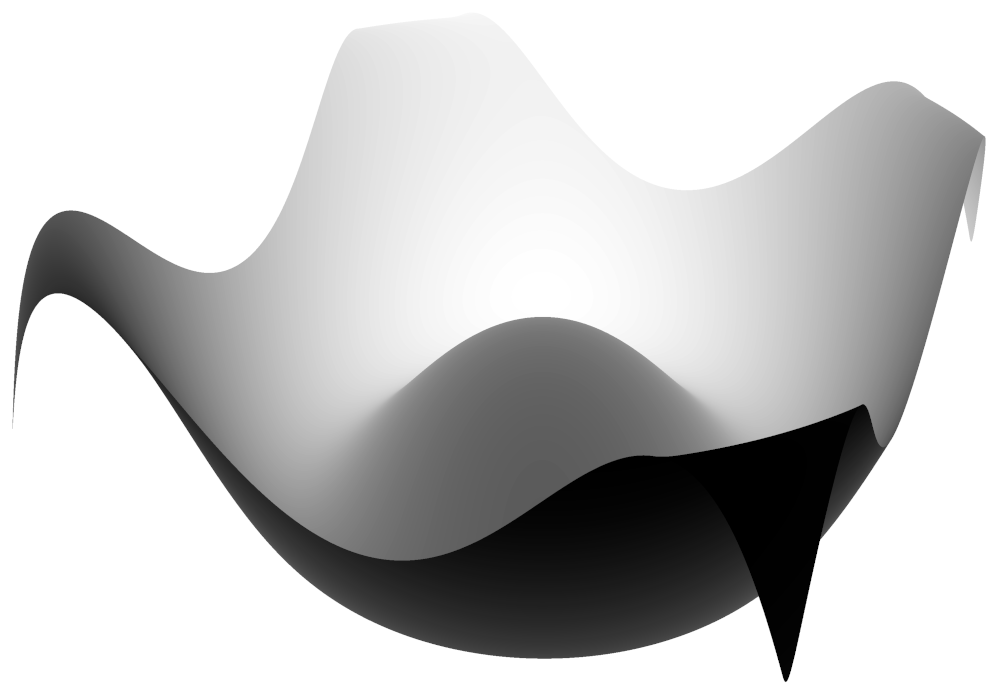
\includegraphics[height=5cm]{images/int_depth.png}
	\caption{Depth (z) pass produced by Cycles. Alpha replaced with black to help visualisation here. Intensity increases with depth from the camera.}\label{int_depth}
\end{figure}

\begin{figure}[h!]
	\centering
	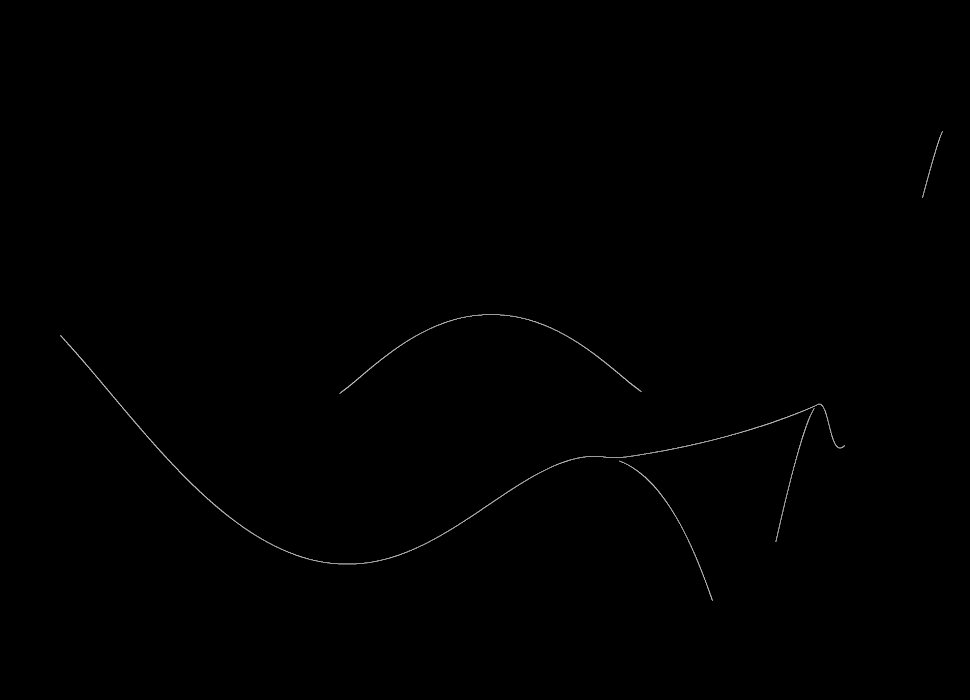
\includegraphics[height=5cm]{images/int_edge.png}
	\caption{Canny edge detection performed on the depth map, using the object index pass as a mask. Result is all edges which do not lie on the Silhouette (i.e. internal edges only.}\label{int_edge}
\end{figure}

\begin{figure}[h!]
	\centering
	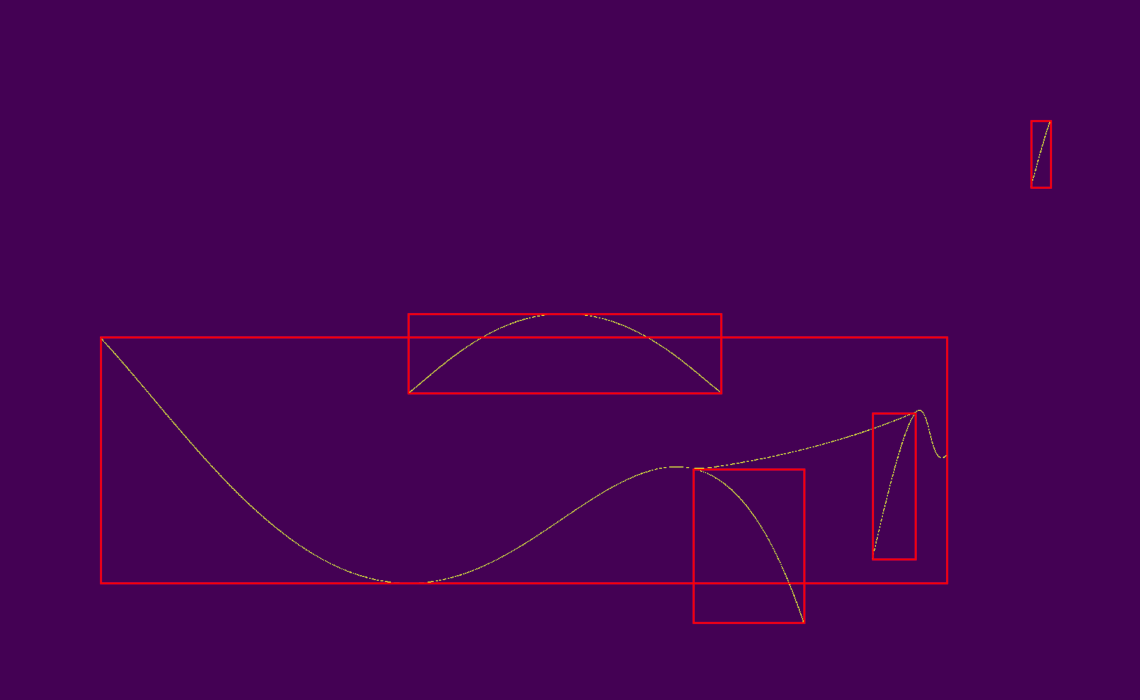
\includegraphics[height=5cm]{images/int_labels.png}
	\caption{Identification of distinct lines using \texttt{skimage.measure.label}. Each line exists in image-space, and must ultimately be converted into a \texttt{Path}, i.e. an \emph{ordered sequence} of image-space coordinates representing the journey along the line.}\label{int_labels}
\end{figure}

\begin{figure}[h!]
	\centering
	\includesvg[height=5cm]{images/int.svg}
	\caption{\texttt{Path}s converted to \texttt{CurvedStroke}s, and rendered as a SVG. Image shows Internal Edges combined with Silhouette.}\label{int}
\end{figure}

\FloatBarrier
\section{Streamlines}\label{impl_stream}
\begin{figure}[h!]
	\centering
	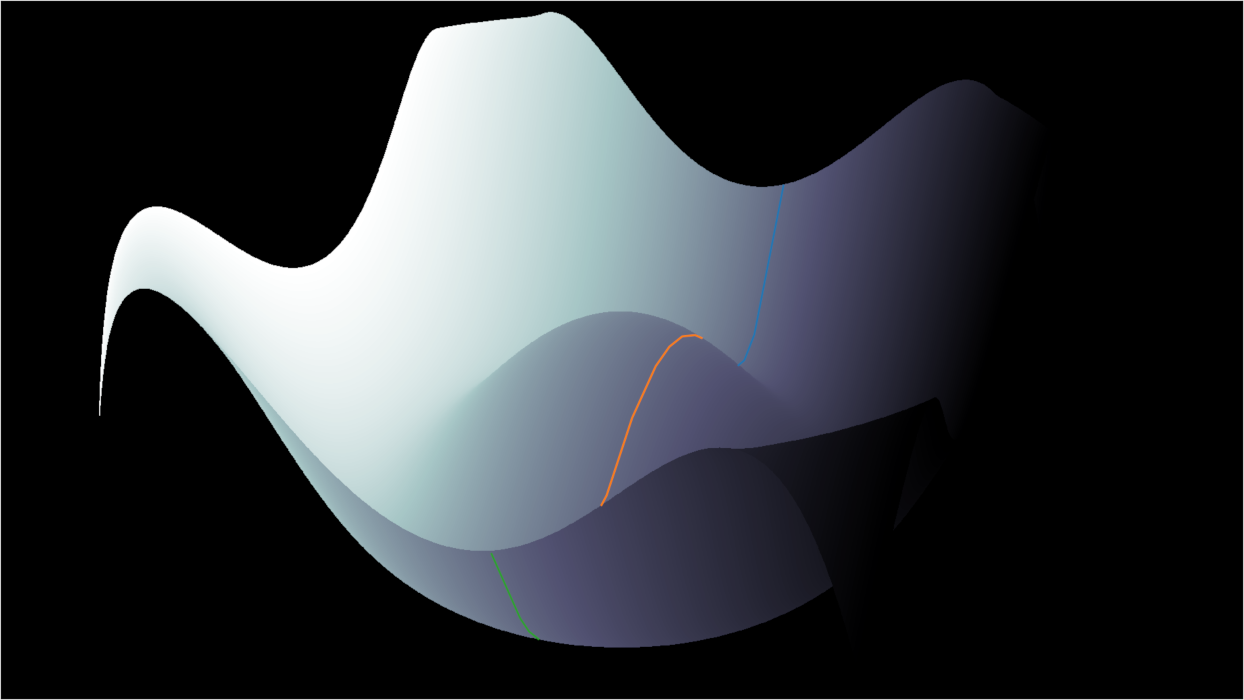
\includegraphics[height=5cm]{images/stream_cont1.png}
	\caption{The surface displayed is an intensity map extracted from Blender's UV pass. This particular image represents the U-coordinate intensities. Streamlines are displayed in colour - these are isolines which follow a given intensity of the underlying surface, creating an effective way to show surface structure. Each isoline is an individual \texttt{Path}. This process is repeated with a range of different intensities in U and V coordinate space, to produce \texttt{Path}s which criss-cross the surface.}\label{stream_cont1}
\end{figure}

\begin{figure}[h!]
	\centering
	
\includegraphics[height=5cm]{images/stream_cont2.png}
	\caption{A further example, with the isoline following a different intensity value.}\label{stream_cont1}
\end{figure}

\begin{figure}[h!]
	\centering
	\includesvg[height=5cm]{images/stream.svg}
	\caption{\texttt{Path}s converted to \texttt{CurvedStroke}s, and rendered as a SVG. Image shows Streamlines combined with Internal Edges and Silhouette.}\label{stream}
\end{figure}

\FloatBarrier
\section{Stipples}\label{impl_stipples}
\begin{figure}[h!]
	\centering
	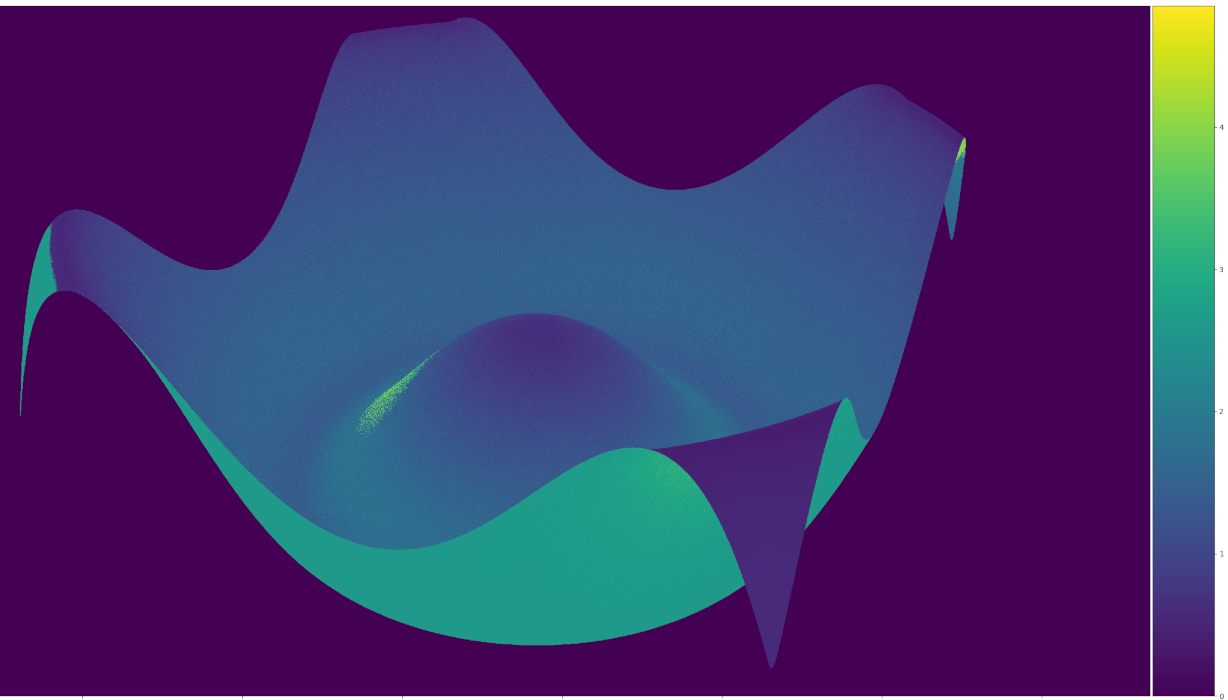
\includegraphics[height=4.5cm]{images/stipple_intensity.png}
	\caption{An intensity map is created, based on a weighted combination of Blender's Direct Diffuse, Ambient Occlusion and Shadow passes. The User is able to control the weight of each, based on which of these components they wish to emphasise in the final render.}\label{stipple_intensity}
\end{figure}

\begin{figure}[h!]
	\centering
	
\includegraphics[height=5cm]{images/stipple_placement.png}
	\caption{Stipple placement locations (nodes) computed by a third party library based on variable density Voroni cells, using the image intensity map (and some further User-provided factors) as the density function. Nodes beyond a User-specified are rejected. Remaining nodes are plotted here for visualisation, each dot represents the ``head'' location for each stipple.}\label{stipple_placement}
\end{figure}

\begin{figure}[h!]
	\centering
	\includesvg[height=5cm]{images/stipple.svg}
	\caption{Each stipple placement coordinate converted to a \texttt{DirectionalStippleStroke}, and rendered as a SVG. Stipples have a ``tail'' which provide insight to underlying structure - the tail is aligned according to the underlying U-coordinate direction of the surface. Image shows Stipples combined with Internal Edges and Silhouette.}\label{stipple}
\end{figure}

\FloatBarrier
\section{Continuous Strokes}

\begin{figure}[h!]
	\centering
	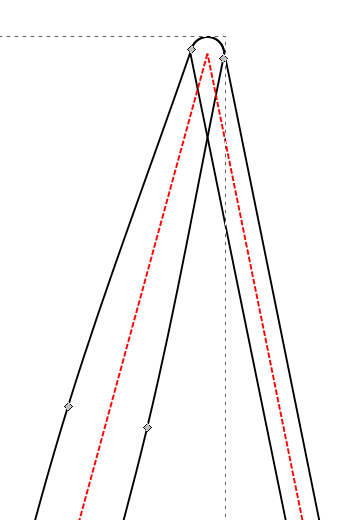
\includegraphics[height=5cm]{images/stroke_construction.png}
	\caption{Anatomy of continuous \texttt{CurvedStroke}s. Image shows clean combination of two strokes. Stroke outlines in black, with no fill applied to aid visualisation. Red dashed lines represent construction curves, from which the black outlines are derived through curve offsetting. Grey control points allow the length of each black outline path allow the stroke thickness to varied over its length (a slight taper is shown here on the leftmost stroke).}\label{stroke_construction}
\end{figure}

\FloatBarrier
\section{Discrete Strokes}

\begin{figure}[h!]
	\centering
	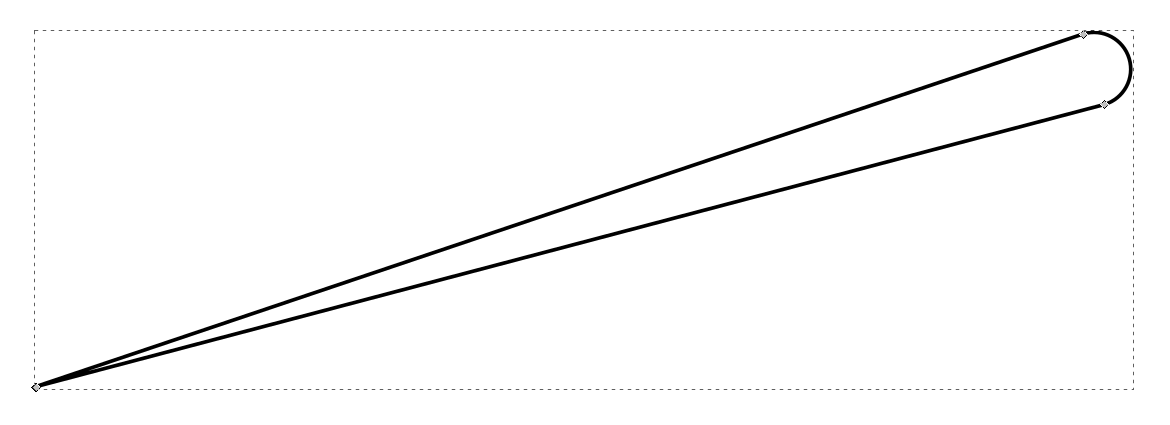
\includegraphics[height=5cm]{images/stipple_construction.png}
	\caption{Anatomy of a discrete \texttt{DirectionalStippleStroke}. Stroke outline in black, with no fill applied to aid visualisation. The radius of the ``tail'' end is set much smaller than the ``head'', to give a severe tapering style.}\label{stroke_construction}
\end{figure}